This section discusses how each database performed on implementing the kernels mentioned in Section \ref{sec:kernels}.

\subsection{Kate's Restaurant Recommendation}

\todo{Discuss the performance results}

\todo{Show scatter plot with each load on x-axis and database as each point on the legend}

Figure \ref{fig:kateResult} shows which restaurants would be recommended to Kate. One can see that both positive sentiment and star average over reviews for highly regarded restaurants compare well and remain consistent.

The reviews returned by the query were typically well above 3 stars and, since the Na\"ive Bayes performed well when predicting unseen text data, it comes as no surprise that most of the reviews were tagged as positive. Further analysis could look at how positive sentiment and star rating would compare for inconsistently performing restaurants but a special measure would need to be put in place to determine how ``inconsistency'' is measured.

\begin{figure}[ht]
    \small
    \centering
    \begin{tabular}{ |p{3.25cm}||p{1.78cm}|p{1.59cm}|}
        \hline
        \rowcolor{Gray}
        \multicolumn{3}{|c|}{Businesses in Phoenix 2018} \\
        \hline
        \rowcolor{LightGray}
        Name & Pos Sentiment & Star Average                 \\
        \hline
        Paco's Tacos \& Tequila     & 92.9825\%  & 4.5833 \\
        Oak Steakhouse Charlotte    & 100.0\%    & 5.0 \\
        The Cheesecake Factory      & 100.0\%    & 4.4615 \\
        Block \& Grinder            & 90.0\%     & 4.3333 \\
        Best Wok                    & 100.0\%    & 4.2 \\
        \hline
    \end{tabular}
    \vspace*{5mm}
    \caption{The result of analysis on the review data of recommended restaurants. Only results with 5 reviews or more are displayed.}
    \label{fig:kateResult}
\end{figure}

\subsection{Review Trends in Phoenix 2018}
\label{sec:resultReviews2018}

\todo{Discuss the performance results}

\todo{Show scatter plot with each load on x-axis and database as each point on the legend}

The general trends shown in review data for Phoenix during 2018 have the following characteristics:

\begin{itemize}
    \item More critical, lower scoring reviews tend to be longer and most useful.
    \item Reviews with 3 or 4 stars seem to be the funniest.
    \item Reviews with 4 or 5 stars tend to be the coolest.
\end{itemize}

The percentage positive sentiment, when scored relatively, is ordered consistently with the average star rating. This validates the performance of the binary sentiment classifier in that one almost does not need to see the star rating and can rely on text data alone when considering a broad spectrum of reviews.

This analysis could then be performed over varied year brackets and different areas to see if performance is consistent or not. The implication of this could lead to experimenting with more sophisticated machine learning models on the dataset to be more precising in that it could potentially predict the star rating as is done in \cite{reddy2017prediction} and \cite{monett2016predicting}.

\begin{figure}[h]
    \centering
    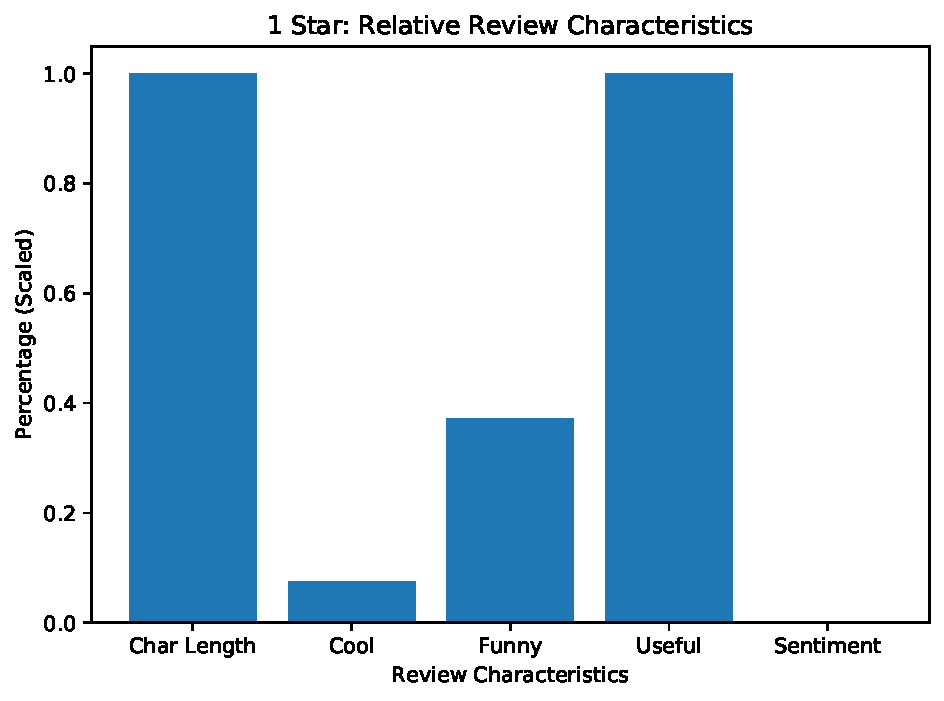
\includegraphics[width=0.49\textwidth]{img/phoenix2018/1Star.pdf}
    \caption{Relative characteristics of 1 star reviews over reviews of restaurants in Phoenix 2018.}
    \label{fig:1star}
\end{figure}

\begin{figure}[h]
    \centering
    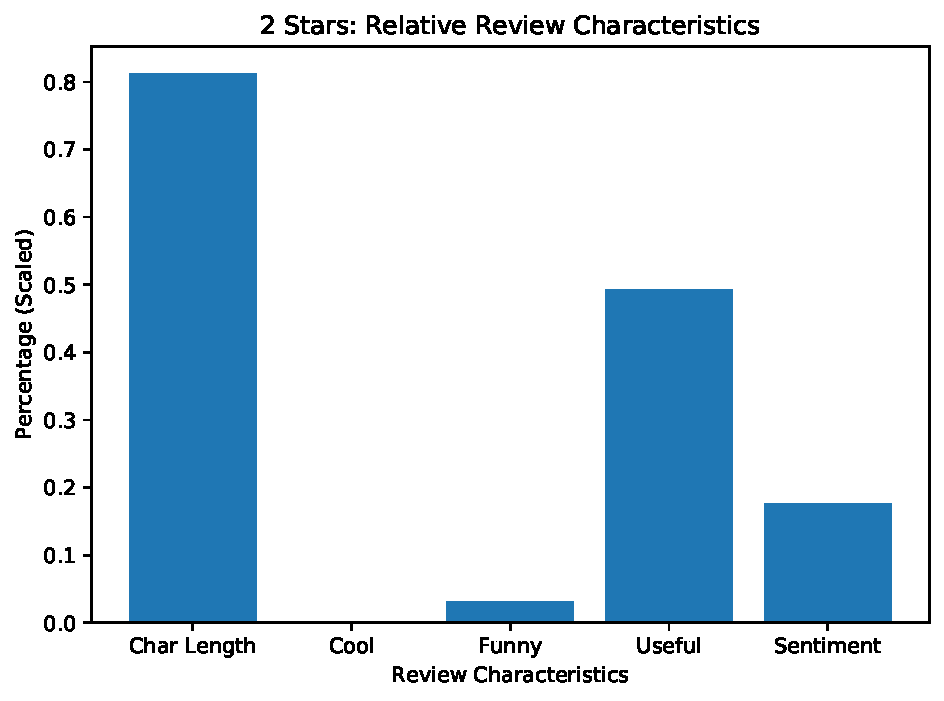
\includegraphics[width=0.49\textwidth]{img/phoenix2018/2Stars.pdf}
    \caption{Relative characteristics of 2 star reviews over reviews of restaurants in Phoenix 2018.}
    \label{fig:2star}
\end{figure}

\begin{figure}[h]
    \centering
    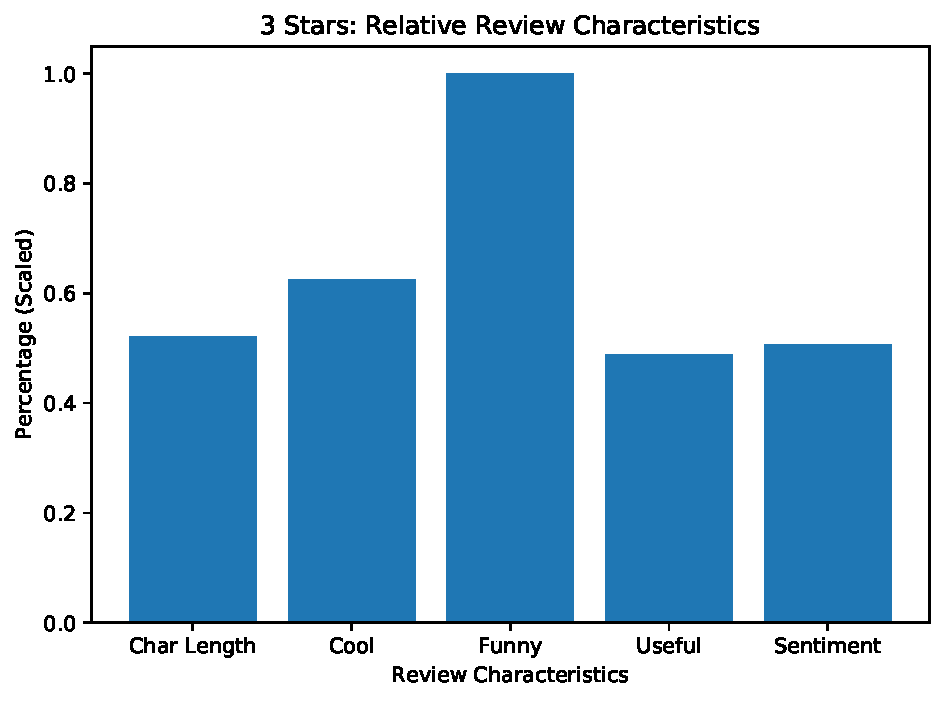
\includegraphics[width=0.49\textwidth]{img/phoenix2018/3Stars.pdf}
    \caption{Relative characteristics of 3 star reviews over reviews of restaurants in Phoenix 2018.}
    \label{fig:3star}
\end{figure}

\begin{figure}[h]
    \centering
    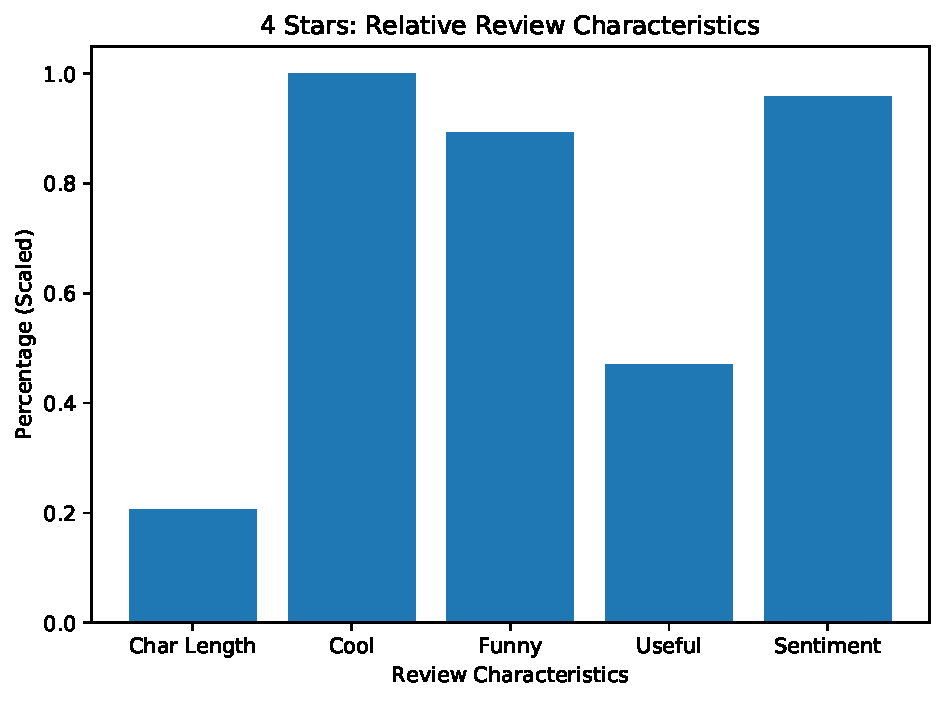
\includegraphics[width=0.49\textwidth]{img/phoenix2018/4Stars.pdf}
    \caption{Relative characteristics of 4 star reviews over reviews of restaurants in Phoenix 2018.}
    \label{fig:4star}
\end{figure}

\begin{figure}[h]
    \centering
    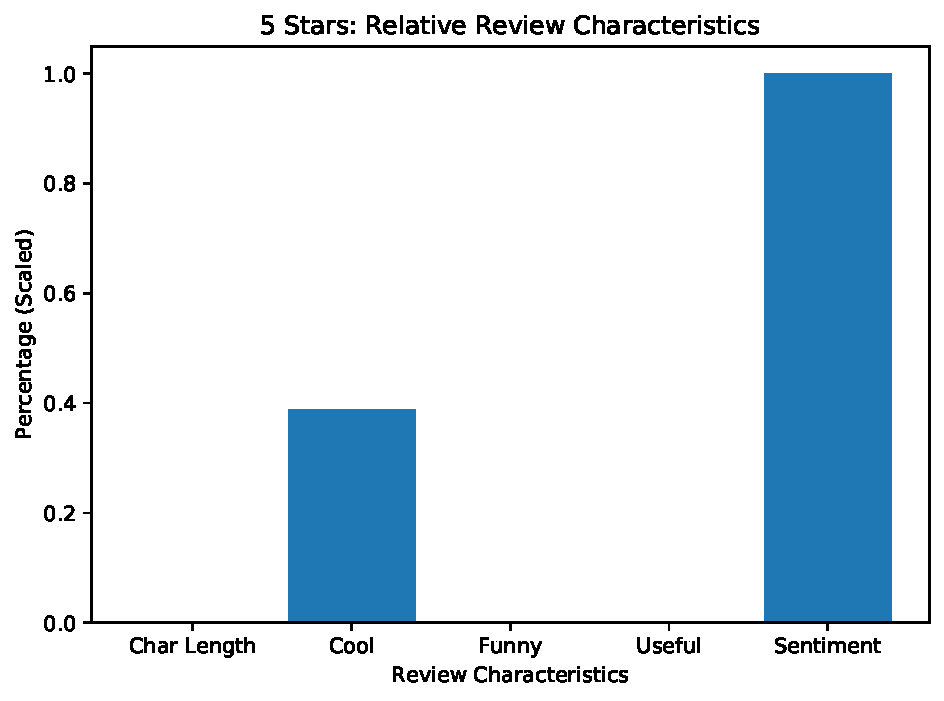
\includegraphics[width=0.49\textwidth]{img/phoenix2018/5Stars.pdf}
    \caption{Relative characteristics of 5 star reviews over reviews of restaurants in Phoenix 2018.}
    \label{fig:5star}
\end{figure}

\subsection{Ranking Las Vegas by Friends' Sentiment}

\todo{Discuss the performance results}

\todo{Show scatter plot with each load on x-axis and database as each point on the legend}

The result of this analysis was focused more on the performance rather than the data extracted. The results of the data analysis on this kernel does not show anything more interesting about the review data than what was already discussed in Section \ref{sec:resultReviews2018}. One notable difference in this kernel however, is that it produces a much more complex query and the databases perform accordingly.

The result of this kernel is simply to show that the results may vary and can be correlated depending on the relationships between different data points.

\begin{figure}[ht]
    \small
    \centering
    \begin{tabular}{ |p{3.5cm}|p{3.5cm}|}
        \hline
        \rowcolor{Gray}
        \multicolumn{2}{|c|}{Las Vegas Sentiment vs Star Average} \\
        \hline
        \rowcolor{LightGray}
        Positive Sentiment (\%) & Star Average \\
        \hline
        70.7767 & 3.8917 \\
        \hline
    \end{tabular}
    \vspace*{5mm}
    \caption{The result of analysis on the review data of Julie's friends.}
    \label{fig:cityResult}
\end{figure}
